\documentclass[11pt,a4paper]{article}

\usepackage[T1]{fontenc}
\usepackage[utf8]{inputenc}
\usepackage{lmodern}
\usepackage[a4paper,margin=2.5cm]{geometry}
\usepackage{graphicx}
\usepackage{microtype}
\usepackage[dvipsnames]{xcolor}
\usepackage[round,authoryear]{natbib}
\usepackage[hidelinks]{hyperref}
\usepackage{parskip}

\definecolor{accent}{HTML}{0D9488}
\hypersetup{colorlinks=true, linkcolor=accent, urlcolor=accent, citecolor=accent}

\title{\textbf{Designing and Building a Computer Science Portfolio}}
\author{Mert \textcolor{accent}{Çelik}\\[2pt]
  \small B.Sc. Software Engineering, GISMA University of Applied Sciences, Berlin}
\date{June 2026}

\begin{document}
\maketitle

\begin{abstract}
\noindent This report explains how I designed and built my computer science portfolio for a working-student (\textit{Werkstudent}) application in Berlin. The portfolio has three parts: a website on GitHub Pages, a one-page CV made with \LaTeX{}, and this report. Below I describe how the website and its repository are organised, explain the main design choices and why I made them, list the tools I used, and look back at what works well, what does not, and what I would like to add later.
\end{abstract}

\section{Introduction}
You can find the live site at \href{https://sw3do.github.io}{https://sw3do.github.io} and the source code at \href{https://github.com/sw3do/sw3do.github.io}{github.com/sw3do/sw3do.github.io}. The goal is simple: to show a hiring manager what I can actually build, for a working-student role in Berlin.

The main thing I kept in mind was time. A hiring manager usually spends less than a minute on a first look at someone's application \citep{pestoPortfolio}, so I tried to make everything quick to read, while still rewarding a closer look. The rest of this report covers the structure of the site and repository (Section~\ref{sec:structure}), the main design decisions and why I made them (Section~\ref{sec:decisions}), the tools I used (Section~\ref{sec:tools}), and an honest look at the strengths and weaknesses (Section~\ref{sec:reflection}).

\section{Portfolio and Repository Structure}
\label{sec:structure}

\subsection{The website}
The site is one scrollable page with a few extra sub-pages. The main page is split into clear sections (Hero, About, Skills, Projects, Experience and Contact) so a reader can find anything quickly. The hero at the top has a short intro and a small terminal panel that lists my main tech, which also fits the systems side of my work.

There are two kinds of sub-page, so the main page does not get crowded. The case studies (for example \texttt{/projects/packet-sniffer} and \texttt{/projects/jikan-rs}) all follow the same simple structure: the problem, what I did and why, a real problem I ran into, the result, and what I would improve next. A small blog holds short notes about the same projects. I only feature public repositories, so every repo and demo link a visitor clicks actually works.

\subsection{The repository}
I organised the repository so that files which change together stay together:

\begin{quote}\small\ttfamily
sw3do.github.io/\\
\hspace*{1em}src/\\
\hspace*{2em}components/  layouts/  pages/\\
\hspace*{2em}content/     (projects + blog, as Markdown)\\
\hspace*{2em}data/        (profile, skills, projects)\\
\hspace*{2em}styles/      (design tokens + global CSS)\\
\hspace*{1em}public/      (CV PDF, OG image, favicon, robots.txt)\\
\hspace*{1em}cv/          (LaTeX source + Mert-Celik-CV.pdf)\\
\hspace*{1em}report/      (this report)\\
\hspace*{1em}.github/workflows/  (build + deploy)\\
\hspace*{1em}README.md
\end{quote}

The site is data-driven on purpose. My profile, skill groups and project list live in typed data files, and the case studies and blog posts are Markdown files in Astro \textit{content collections}. The components just read from these, so changing the content never means touching the layout code. This keeps each file small and the project easy to extend.

\section{Design Decisions and Justification}
\label{sec:decisions}

\subsection{One look across everything}
The CV, the website and this report all share the same simple look: one teal accent colour, a small set of fonts, and a clean layout with plenty of space. Using the same style everywhere helps a reader see them as one piece of work, and keeping it minimal puts the important things near the top, where a busy reader will actually see them \citep{scrimbaPortfolio, pestoPortfolio}.

\subsection{A one-page, single-column, ATS-safe CV}
The CV is a single page in one column. For a student this is the format most guides recommend: it makes you keep only the best things, and it survives the automated applicant-tracking systems (ATS) that get confused by multi-column layouts \citep{techinterviewhandbook, jobshinobi2026}. I put skills and projects first instead of work history, because as a student my public projects are really my experience \citep{uwcareers2025}. The bullet points try to say what I did, with which technology, and what came out of it, instead of just listing tasks \citep{igotanoffer}. I compile it with \texttt{pdfLaTeX} and a \texttt{glyphtounicode} mapping, so the PDF text can still be selected and copied cleanly \citep{jakesresume, atsresumeai}.

\subsection{An anonymous CV for the Berlin market}
The CV has no photo, date of birth or home address. A photo is still common in German applications, but the anonymous CV is becoming normal, especially in Berlin's international, English-speaking tech scene, and it leaves less room for bias \citep{cvcompose2026}. I give my language levels on the CEFR scale and list German honestly at A1, with a note that I am still learning it. German employers seem to value that kind of honesty \citep{goetheCV, werkstudent2026}.

\subsection{A static site with Astro}
The website is a static site built with Astro and deployed with GitHub Actions. By default Astro sends almost no JavaScript to the browser, which helps a lot with the speed and accessibility goals below, and its content collections make the case studies and blog easy to write and check \citep{astroDocs}. A static build also fits GitHub Pages well and gives me an automatic deploy every time I push.

\subsection{Accessibility, performance and SEO}
The site uses semantic HTML with a proper heading order, clear labels and visible keyboard focus, and I aimed for WCAG AA colour contrast in both the dark and light themes. This helps accessibility, and since the same things feed into Google's Core Web Vitals, it also helps search ranking and how good the site feels \citep{siteimproveCWV, owdt}. The layout is mobile-first, because Google indexes the mobile version and a lot of people will open the link on their phone \citep{engagecoders}. GitHub Pages cannot run any server code, so I add the search and social data at build time: per-page titles and descriptions, Open Graph and Twitter cards, JSON-LD data, a sitemap and a \texttt{robots.txt} \citep{jekyllpadSEO}.

\subsection{Honesty over polish}
Every project I show is real, and each case study names a real problem I had and an honest ``what I would improve next''. Vague claims with no detail are exactly the kind of thing that makes a portfolio look fake or AI-written \citep{learnist}, so I tried to keep the text specific and honest instead of decorative.

\section{Tools and Technologies}
\label{sec:tools}
\begin{itemize}
\item \textbf{Astro + TypeScript} --- static site generation with typed data and content collections.
\item \textbf{CSS custom properties} --- one source of truth for the dark and light design tokens.
\item \textbf{astro-icon} with \textbf{Lucide} and \textbf{Simple Icons} --- accessible SVG icons inlined at build time.
\item \textbf{@fontsource} (Space Grotesk, Inter, JetBrains Mono) --- self-hosted fonts, so the build works offline and stays fast.
\item \textbf{@astrojs/sitemap} --- generates the sitemap automatically.
\item \textbf{GitHub Pages + GitHub Actions} --- hosting, and a deploy on every push.
\item \textbf{Git} --- version control.
\item \textbf{\LaTeX} (\texttt{pdfLaTeX}, \texttt{lmodern}, \texttt{natbib}, \texttt{glyphtounicode}) --- the CV and this report.
\item \textbf{Pillow} --- generating the social-share (Open Graph) image in code.
\item \textbf{Google Lighthouse} --- checking performance, accessibility, best practices and SEO.
\end{itemize}

I kept the toolchain small and portable on purpose. The documents compile with a basic \LaTeX{} install and no extra citation program, and the site builds with a single \texttt{npm} command.

\section{Reflection}
\label{sec:reflection}

\subsection{Strengths}
I think the portfolio shows a decent range and some depth. There are real projects in Rust, Go, Python and TypeScript: a published library, a networking tool, a small machine-learning service, and a cross-platform desktop app. A lot of the quality can be measured instead of just claimed, since the site is accessible, fast and set up for search. The CV, website and report also look like one consistent thing, the deploy happens automatically, and the CV is properly ATS-safe.

\subsection{Weaknesses}
My formal work experience is still limited, and a few of the projects are libraries or command-line tools with no live demo, which is harder to show off than an interactive web app. My German is only A1. The site has no automated tests, and since I worked on it alone, nobody else has reviewed the code.

\subsection{Future work}
There are a few things I would like to add. Real numbers for each project (benchmarks, test coverage, download counts), more case studies, a custom domain, automatic link-checking and Lighthouse runs in CI so things do not break, support for more languages (English, German and Turkish), and a more active blog. Adding live demos for the library and CLI projects, maybe a small playground, would also make a better first impression.

\begingroup
\raggedright
\begin{thebibliography}{99}
\bibitem[ATS Resume AI(2026)]{atsresumeai} ATS Resume AI. 2026. \textit{ATS resume formatting rules: font size, margins and spacing}. [Online]. Available at: \url{https://www.atsresumeai.com/blog/ats-resume-formatting-guide} [Accessed 5 June 2026].
\bibitem[Astro(2026)]{astroDocs} Astro. 2026. \textit{Astro documentation}. [Online]. Available at: \url{https://docs.astro.build/} [Accessed 5 June 2026].
\bibitem[BeamJobs(2026)]{beamjobs2026} BeamJobs. 2026. \textit{Software engineer resume examples and guide for 2026}. [Online]. Available at: \url{https://www.beamjobs.com/resumes/software-engineer-resume-examples} [Accessed 5 June 2026].
\bibitem[CVCompose(2026)]{cvcompose2026} CVCompose. 2026. \textit{Personal details in your CV 2026: photo, age, address and GDPR}. [Online]. Available at: \url{https://cvcompose.com/blog/personal-data-cv-2026-gdpr-photo} [Accessed 5 June 2026].
\bibitem[EngageCoders(2025)]{engagecoders} EngageCoders. 2025. \textit{Mobile-first responsive website: best practices}. [Online]. Available at: \url{https://www.engagecoders.com/responsive-web-design-mobile-first-development-best-practices-2025-guide/} [Accessed 5 June 2026].
\bibitem[Goethe-Institut(2024)]{goetheCV} Goethe-Institut. 2024. \textit{Classifying knowledge of German on a CV}. [Online]. Available at: \url{https://www.goethe.de/ins/in/en/spr/mag/20629104.html} [Accessed 5 June 2026].
\bibitem[Gutierrez(2024)]{jakesresume} Gutierrez, J. 2024. \textit{Jake's resume}. [Online]. Available at: \url{https://github.com/jakegut/resume} [Accessed 5 June 2026].
\bibitem[IGotAnOffer(2025)]{igotanoffer} IGotAnOffer. 2025. \textit{Google resume examples and optimization tips}. [Online]. Available at: \url{https://igotanoffer.com/blogs/tech/google-resume-examples-tips} [Accessed 5 June 2026].
\bibitem[JekyllPad(2025)]{jekyllpadSEO} JekyllPad. 2025. \textit{Mastering SEO for GitHub Pages}. [Online]. Available at: \url{https://www.jekyllpad.com/blog/mastering-github-pages-seo-7} [Accessed 5 June 2026].
\bibitem[Job Shinobi(2026)]{jobshinobi2026} Job Shinobi. 2026. \textit{Is a \LaTeX{} resume ATS friendly?} [Online]. Available at: \url{https://www.jobshinobi.com/blog/is-a-latex-resume-ats-friendly-2026} [Accessed 5 June 2026].
\bibitem[Learnist(2026)]{learnist} Learnist. 2026. \textit{Red flags in AI case studies}. [Online]. Available at: \url{https://www.learnist.org/ai-case-study-red-flags-portfolio-2026/} [Accessed 5 June 2026].
\bibitem[OWDT(2025)]{owdt} OWDT. 2025. \textit{How to improve Core Web Vitals: a complete guide}. [Online]. Available at: \url{https://owdt.com/insight/how-to-improve-core-web-vitals/} [Accessed 5 June 2026].
\bibitem[Pesto(2025)]{pestoPortfolio} Pesto. 2025. \textit{What recruiters look for in developer portfolios}. [Online]. Available at: \url{https://pesto.tech/resources/what-recruiters-look-for-in-developer-portfolios} [Accessed 5 June 2026].
\bibitem[Scrimba(2025)]{scrimbaPortfolio} Scrimba. 2025. \textit{How to build a web developer portfolio that gets you hired}. [Online]. Available at: \url{https://scrimba.com/articles/how-to-build-a-web-developer-portfolio-that-gets-you-hired/} [Accessed 5 June 2026].
\bibitem[Siteimprove(2025)]{siteimproveCWV} Siteimprove. 2025. \textit{Core Web Vitals and WCAG}. [Online]. Available at: \url{https://www.siteimprove.com/blog/core-web-vitals-wcag/} [Accessed 5 June 2026].
\bibitem[Study-Abroad.org(2026)]{werkstudent2026} Study-Abroad.org. 2026. \textit{Werkstudent guide: working student jobs in Germany}. [Online]. Available at: \url{https://www.study-abroad.org/blog/werkstudent-guide-international-students-germany/} [Accessed 5 June 2026].
\bibitem[Tech Interview Handbook(2025)]{techinterviewhandbook} Tech Interview Handbook. 2025. \textit{Resume guide}. [Online]. Available at: \url{https://www.techinterviewhandbook.org/resume/} [Accessed 5 June 2026].
\bibitem[University of Washington(2025)]{uwcareers2025} University of Washington Career Center. 2025. \textit{Entry-level software engineer resume: what recruiters want to see}. [Online]. Available at: \url{https://careers.uw.edu/blog/2025/08/01/entry-level-software-engineer-resume-what-recruiters-want-to-see/} [Accessed 5 June 2026].
\end{thebibliography}
\endgroup

\appendix
\section{Lighthouse Audit}
\IfFileExists{assets/lighthouse.png}{%
  \begin{center}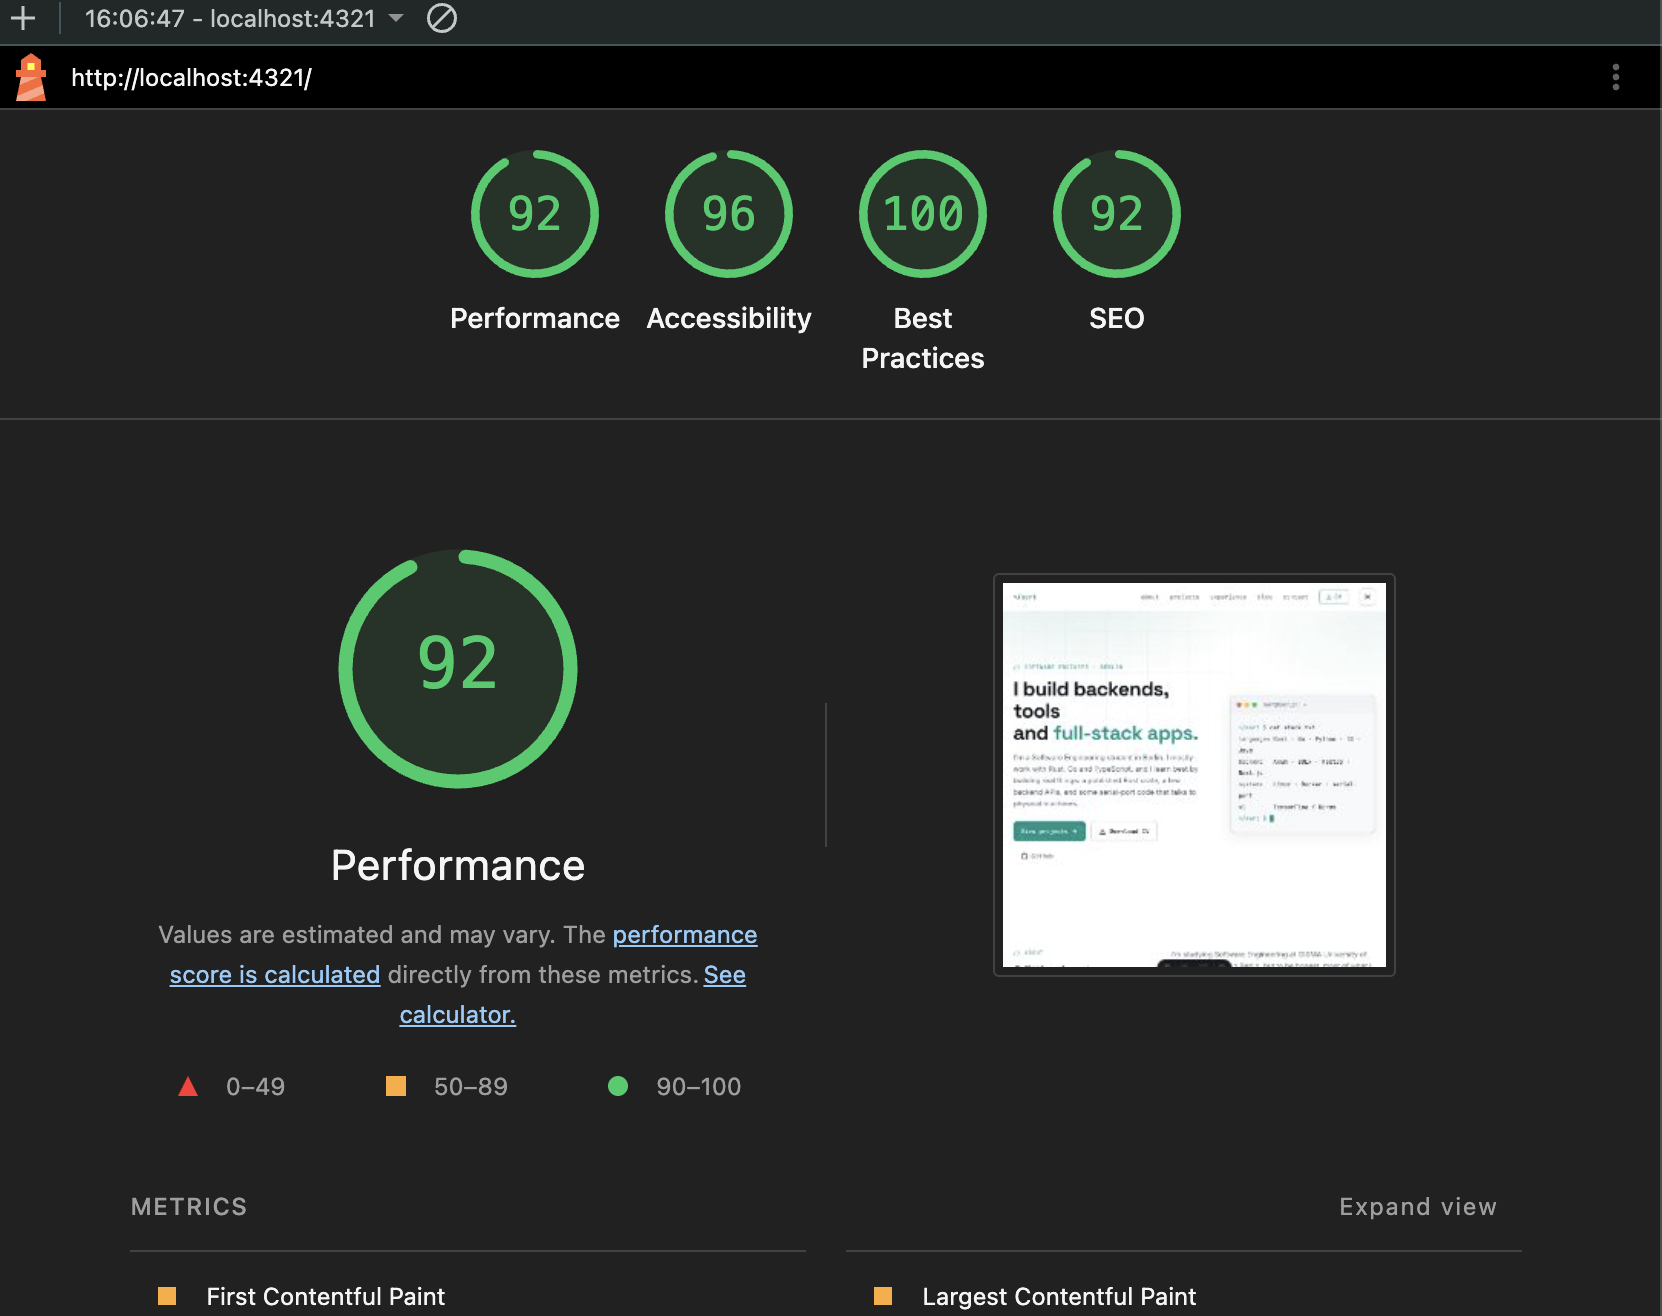
\includegraphics[width=0.85\textwidth]{assets/lighthouse.png}\end{center}%
}{%
  \textit{A Google Lighthouse audit of the deployed site goes here, showing the Performance, Accessibility, Best Practices and SEO scores.}%
}

\end{document}
